%\newpage
\section{Ergebnisse und Berechnungen}
\label{sec:ergebnisse}

\subsection{Allgemeine Daten und Annahmen}
Als allgemeine Daten werden unter diesen Abschnitt Daten aufgeführt, welche lediglich einmalig für das Praktikum bestimmt wurden und nicht mit jeder Messerreihe erneut gemessen (siehe Tab. \ref{tab:allgemein}).

% Table generated by Excel2LaTeX from sheet 'Daten'
\begin{table}[h!]
	\renewcommand*{\arraystretch}{1.2}
	\centering
	\rowcolors{2}{white}{gray!25}
	\caption{Allgemeine Daten}
	\label{tab:allgemein}
	\resizebox{15cm}{!}{
		\begin{tabulary}{1.2\textwidth}{C|C|C}
			\hline
			\textbf{Umgebungsdruck $p_u$ $\left[\si{\bar}\right]$}&\textbf{Rührerdurchmesser $d_R$ $\left[\si{\meter}\right]$} &\textbf{Luftvolumenstrom $\dot{V}$ $\left[\si{\liter \per \minute}\right]$} \\
			\hline
			1,013 & 0,11 & 0,5\\
			\hline			
		\end{tabulary}
	}
\end{table}%
\FloatBarrier

\begin{figure}[h!]
	\centering
	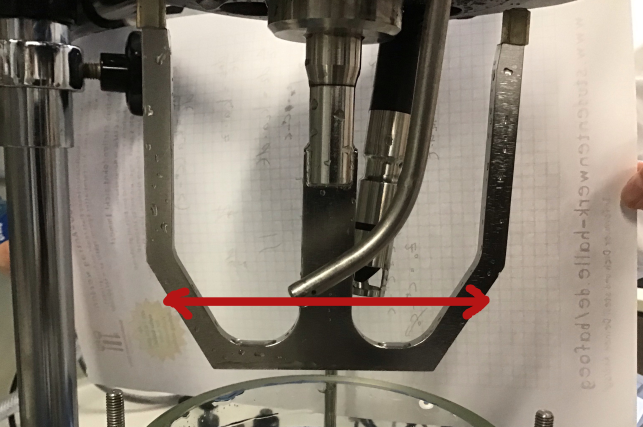
\includegraphics[width=0.35\textwidth]{img/anker}
	\caption{angenommener Durchmesser am Ankerrührer}
	\label{fig:anker}
\end{figure}
\FloatBarrier
%Ende
Der Rührerdurchmesser wird für die Berechnung der Reynoldszahl auf Höhe des einleitenden Gases angenommen (siehe Abb. \ref{fig:anker}).

Ebenfalls werden unter diesem Abschnitt die getroffenen Annahmen für die folgenden Berechnungen aufgeführt (siehe Tab. \ref{tab:annahmen}).

% Table generated by Excel2LaTeX from sheet 'Daten'
\begin{table}[h!]
	\renewcommand*{\arraystretch}{1.2}
	\centering
	\rowcolors{2}{white}{gray!25}
	\caption{Annahmen}
	\label{tab:annahmen}
	\resizebox{15cm}{!}{
		\begin{tabulary}{1.2\textwidth}{C|C|C}
			\hline
			\textbf{Bezeichnung}&\textbf{Annahme}&\textbf{Begründung}\\
			Dichte Wasser & $\rho_{\ce{H2O}} \approx const.$& Wassertemperatur ändert sich unwesentlich ($\Delta T = \SI{0,4}{\kelvin}$)\\
			Viskosität Wasser & $\nu_{\ce{H2O}} \approx const.$& Wassertemperatur ändert sich unwesentlich ($\Delta T = \SI{0,4}{\kelvin}$)\\
			Partialdruck Sauerstoff &  $p^{\ast}_{\ce{O2}}\approx p_{\text{Umgebung}}$ & $\frac{p_{\ce{H2O}}}{p_{\text{Umgebung}}} << 1 \rightarrow$ vernachlässigbar \\
			Sauerstoffanteil & $x_{\ce{O2}} = 0,21$ & realitätsnaher Wert\\
			Stoffmenge & $n_{ges} \approx n_{\ce{H2O}}$ & $\frac{n_{\ce{O2}}}{n_{\ce{H2O}}}<<1 \rightarrow$ vernachlässigbar\\
			\hline			
		\end{tabulary}
	}
\end{table}%
\FloatBarrier

\newpage

\subsection{Messdaten und Berechnungen}
Es wurden für dieses Praktikum drei Messreihen durchgeführt, welche Drehzahlen von \SI{80}{\per \minute}, \SI{110}{\per \minute} und \SI{140}{\per \minute} umfassten. In Abbildung \ref{dia:konzentration} sind zunächst die Konzentrationsverläufe der einzelnen Messreihen dargelegt. Bereits an dieser Stelle fällt auf, dass Messreihe 1 mit \SI{80}{\per \minute} einen abweichenden Kurvenverlauf zu den übrigen Messreihen aufzeigt. Weiterhin erkennbar ist, dass ohne Betrachtung von Messreihe 1, Messreihe 3 mit \SI{140}{\per \minute} den steileren Kurvenverlauf zeigt.
In Gleichung \eqref{gl:umrechnung} ist die Umrechnung der gemessenen Konzentration \si{\milli \gram \per \liter} in \si{\milli \mole \per \liter} zu finden.

\begin{flalign}
	\label{gl:umrechnung}
		c &= \frac{\beta}{M} = \frac{\SI{10}{\gram \per \liter} }{\SI{32}{\gram \per \mole}}  \\
		&= \underline{\SI{0,313}{\mol \per \liter}}
\end{flalign}

\begin{figure}[h!]
	\begin{center}
		\resizebox{0.7\textwidth}{!}{
			\begin{tikzpicture}[trim axis left, trim axis right]
				\begin{axis}[
					grid,
					axis lines = left,
					width = 15cm,
					height = 9cm,
					xmin = 0,
					xmax = 1160,
					ymin = 0,
					ymax = 0.3,
				%	ytick = {0,5,...,60},
				%	xtick = {0,1,2,...,15},
					ylabel={Konzentration in \si{\milli \mol \per \liter}},
					%y label style={at={(0,0.5)}},
					xlabel={Zeit in \si{\second}},
					legend style={at={(0.75,0.5)},anchor=west},
					%	y dir = reverse,
					]			
					
					%80 pro minute
					\addplot [color=black, mark=*, only marks] coordinates{(0,0.039375) (5,0.0459375) (10,0.0521875) (15,0.058125) (20,0.06375) (25,0.069375) (30,0.0753125) (35,0.08125) (40,0.0859375) (45,0.09125) (50,0.0953125) (55,0.1) (60,0.1040625) (65,0.1084375) (70,0.1128125) (75,0.1165625) (80,0.1209375) (85,0.1253125) (90,0.1284375) (95,0.131875) (100,0.1353125) (105,0.13875) (110,0.1421875) (115,0.1453125) (120,0.148125) (125,0.15125) (130,0.1540625) (135,0.1565625) (140,0.1590625) (145,0.161875) (150,0.1646875) (155,0.1665625) (160,0.16875) (165,0.1709375) (170,0.173125) (175,0.175) (180,0.1765625) (185,0.1790625) (190,0.180625) (195,0.1825) (200,0.1840625) (205,0.185625) (210,0.186875) (215,0.18875) (220,0.19) (225,0.19125) (230,0.1921875) (235,0.193125) (240,0.194375) (245,0.195625) (250,0.196875) (255,0.1978125) (260,0.1990625) (265,0.2) (270,0.20125) (275,0.201875) (280,0.2028125) (285,0.20375) (290,0.2046875) (295,0.205625) (300,0.2065625) (305,0.2071875) (310,0.2075) (315,0.2084375) (320,0.209375) (325,0.2103125) (330,0.21125) (335,0.211875) (340,0.2128125) (345,0.2134375) (350,0.2134375) (355,0.214375) (360,0.2153125) (365,0.215625) (370,0.2165625) (375,0.2171875) (380,0.2178125) (385,0.21875) (390,0.219375) (395,0.22) (400,0.220625) (405,0.22125) (410,0.2221875) (415,0.2228125) (420,0.223125) (425,0.2240625) (430,0.2246875) (435,0.225) (440,0.2253125) (445,0.2259375) (450,0.2265625) (455,0.2271875) (460,0.2278125) (465,0.2284375) (470,0.22875) (475,0.23) (480,0.2303125) (485,0.230625) (490,0.23125) (495,0.231875) (500,0.2325) (505,0.233125) (510,0.2334375) (515,0.234375) (520,0.2346875) (525,0.2353125) (530,0.235625) (535,0.23625) (540,0.236875) (545,0.2371875) (550,0.2375) (555,0.238125) (560,0.2384375) (565,0.2390625) (570,0.239375) (575,0.24) (580,0.24) (585,0.24125) (590,0.24125) (595,0.241875) (600,0.2421875) (605,0.2428125) (610,0.2428125) (615,0.24375) (620,0.24375) (625,0.2446875) (630,0.245) (635,0.245) (640,0.24625) (645,0.24625) (650,0.2465625) (655,0.2471875) (660,0.2471875) (665,0.2475) (670,0.2478125) (675,0.24875) (680,0.24875) (685,0.2490625) (690,0.25) (695,0.2496875) (700,0.2503125) (705,0.2509375) (710,0.2509375) (715,0.2515625) (720,0.251875) (725,0.251875) (730,0.2525) (735,0.2528125) (740,0.253125) (745,0.253125) (750,0.2534375) (755,0.2540625) (760,0.2540625) (765,0.255) (770,0.255) (775,0.255) (780,0.2553125) (785,0.255625) (790,0.25625) (795,0.256875) (800,0.256875) (805,0.2575) (810,0.2578125) (815,0.258125) (820,0.2584375) (825,0.2584375) (830,0.25875) (835,0.2590625) (840,0.2590625) (845,0.259375) (850,0.2596875) (855,0.26) (860,0.2603125) (865,0.2609375) (870,0.260625) (875,0.2609375) (880,0.26125) (885,0.261875) (890,0.261875) (895,0.2621875) (900,0.2621875) (905,0.2625) (910,0.263125) (915,0.2634375) (920,0.263125) (925,0.2634375) (930,0.26375) (935,0.2640625) (940,0.264375) (945,0.264375) (950,0.2646875) (955,0.265) (960,0.2653125) (965,0.265625) (970,0.265625) (975,0.2659375) (980,0.2659375) (985,0.26625) (990,0.2665625) (995,0.266875) (1000,0.266875) (1005,0.2671875) (1010,0.2675) (1015,0.2675) (1020,0.2675) (1025,0.2678125) (1030,0.268125) (1035,0.268125) (1040,0.2684375) (1045,0.26875) (1050,0.26875) (1055,0.26875) (1060,0.2690625) (1065,0.269375) (1070,0.269375) (1075,0.2696875) (1080,0.2696875) (1085,0.27) (1090,0.27) (1095,0.27) (1100,0.2709375) (1105,0.270625) (1110,0.2709375) (1115,0.2709375) (1120,0.2709375) (1125,0.27125) (1130,0.2715625) (1135,0.2715625) (1140,0.271875) (1145,0.271875) (1150,0.2721875) (1155,0.2725) };
					
%					%110 pro minute
					\addplot [color=red, mark=*, only marks] coordinates{(0,0.03625) (4,0.03875) (9,0.0415625) (14,0.0446875) (19,0.046875) (24,0.049375) (29,0.051875) (34,0.0546875) (39,0.0575) (44,0.06) (49,0.0625) (54,0.065) (59,0.0675) (64,0.07) (69,0.0725) (74,0.0753125) (79,0.0778125) (84,0.08) (89,0.0825) (94,0.0846875) (99,0.0871875) (104,0.0896875) (109,0.091875) (114,0.0940625) (119,0.0965625) (124,0.0984375) (129,0.1009375) (134,0.103125) (139,0.1053125) (144,0.1071875) (149,0.1090625) (154,0.11125) (159,0.1134375) (164,0.1153125) (169,0.1178125) (174,0.1196875) (179,0.1215625) (184,0.1234375) (189,0.125625) (194,0.1271875) (199,0.12875) (204,0.1309375) (209,0.1328125) (214,0.1346875) (219,0.13625) (224,0.138125) (229,0.14) (234,0.1415625) (239,0.1428125) (244,0.1446875) (249,0.14625) (254,0.148125) (259,0.15) (264,0.15125) (269,0.1528125) (274,0.154375) (279,0.1559375) (284,0.1578125) (289,0.1590625) (294,0.1603125) (299,0.161875) (304,0.1634375) (309,0.165) (314,0.1665625) (319,0.1678125) (324,0.169375) (329,0.170625) (334,0.171875) (339,0.173125) (344,0.1746875) (349,0.1759375) (354,0.1775) (359,0.1784375) (364,0.18) (369,0.1809375) (374,0.1825) (379,0.18375) (384,0.185) (389,0.1865625) (394,0.1871875) (399,0.188125) (404,0.189375) (409,0.190625) (414,0.191875) (419,0.1928125) (424,0.1940625) (429,0.195) (434,0.1959375) (439,0.1971875) (444,0.198125) (449,0.1990625) (454,0.2003125) (459,0.20125) (464,0.2021875) (469,0.203125) (474,0.2040625) (479,0.2053125) (484,0.2065625) (489,0.2075) (494,0.2084375) (499,0.2090625) (504,0.2096875) (509,0.2109375) (514,0.2115625) (519,0.2125) (524,0.21375) (529,0.214375) (534,0.215) (539,0.2159375) (544,0.216875) (549,0.2178125) (554,0.2184375) (559,0.22) (564,0.220625) (569,0.2209375) (574,0.2215625) (579,0.2221875) (584,0.2234375) (589,0.224375) (594,0.225) (599,0.225625) (604,0.2259375) (609,0.226875) (614,0.2275) (619,0.2284375) (624,0.2290625) (629,0.2296875) (634,0.230625) (639,0.2309375) (644,0.231875) (649,0.2325) (654,0.2328125) (659,0.23375) (664,0.2346875) (669,0.235) (674,0.235625) (679,0.23625) (684,0.236875) (689,0.2375) (694,0.238125) (699,0.238125) (704,0.23875) (709,0.239375) (714,0.24) (719,0.2403125) (724,0.2409375) (729,0.2415625) (734,0.2421875) (739,0.2425) (744,0.24375) (749,0.2440625) (754,0.2440625) (759,0.244375) (764,0.2453125) (769,0.245625) (774,0.24625) (779,0.2465625) (784,0.246875) (789,0.2471875) (794,0.248125) (799,0.2484375) (804,0.24875) (809,0.2490625) (814,0.2496875) (819,0.25) (824,0.250625) (829,0.2509375) (834,0.2515625) (839,0.2515625) (844,0.2521875) (849,0.2528125) (854,0.2534375) (859,0.25375) (864,0.2540625) (869,0.254375) (874,0.254375) (879,0.255) (884,0.2559375) (889,0.2559375) (894,0.25625) (899,0.256875) (904,0.256875) (909,0.2571875) (914,0.2578125) (919,0.258125) (924,0.2578125) (929,0.2584375) (934,0.25875) (939,0.259375) (944,0.2596875) (949,0.2596875) (954,0.2603125) (959,0.2603125) (964,0.260625) (969,0.260625) (974,0.2615625) (979,0.2621875) (984,0.2621875) (989,0.2628125) (994,0.2628125) (999,0.2634375) (1004,0.2634375) (1009,0.26375) (1014,0.26375) (1019,0.2640625) (1024,0.2646875) (1029,0.2646875) (1034,0.265) (1039,0.2653125) (1044,0.2653125) (1049,0.2659375) (1054,0.26625) (1059,0.2665625) (1064,0.2665625) (1069,0.266875) (1074,0.266875) (1079,0.2678125) (1084,0.268125) (1089,0.2678125) (1094,0.268125) (1099,0.2684375) (1104,0.26875) (1109,0.2690625) (1114,0.2690625) (1119,0.269375) (1124,0.269375) (1129,0.269375) (1134,0.27) (1139,0.2703125) (1144,0.2703125) (1149,0.2703125) (1154,0.2709375) (1159,0.27125) (1164,0.27125) (1169,0.2715625) (1174,0.2715625) (1179,0.2715625) (1184,0.2721875) (1189,0.2725) (1194,0.2725) (1199,0.2728125) (1204,0.2728125) (1209,0.273125) (1214,0.2734375) (1219,0.273125) (1224,0.273125) (1229,0.2734375) (1234,0.2740625) (1239,0.2740625) (1244,0.274375) };
%					
%					%140 pro minute
					\addplot [color=blue, mark=*, only marks] coordinates{(0,0.0328125) (5,0.03625) (10,0.0390625) (15,0.0425) (20,0.045625) (25,0.0490625) (30,0.0521875) (35,0.055625) (40,0.05875) (45,0.0621875) (50,0.065) (55,0.068125) (60,0.0715625) (65,0.074375) (70,0.0775) (75,0.0803125) (80,0.0834375) (85,0.0865625) (90,0.0890625) (95,0.091875) (100,0.0946875) (105,0.0975) (110,0.1) (115,0.1025) (120,0.1053125) (125,0.108125) (130,0.110625) (135,0.1134375) (140,0.115625) (145,0.118125) (150,0.120625) (155,0.1228125) (160,0.125625) (165,0.1275) (170,0.13) (175,0.1325) (180,0.1346875) (185,0.136875) (190,0.1390625) (195,0.1409375) (200,0.143125) (205,0.145) (210,0.1471875) (215,0.149375) (220,0.15125) (225,0.1534375) (230,0.1553125) (235,0.1571875) (240,0.1590625) (245,0.1609375) (250,0.1625) (255,0.164375) (260,0.16625) (265,0.168125) (270,0.1696875) (275,0.1715625) (280,0.173125) (285,0.175) (290,0.1765625) (295,0.1778125) (300,0.1796875) (305,0.18125) (310,0.183125) (315,0.1846875) (320,0.1859375) (325,0.1871875) (330,0.18875) (335,0.19) (340,0.1915625) (345,0.193125) (350,0.1940625) (355,0.1953125) (360,0.1971875) (365,0.1984375) (370,0.1996875) (375,0.20125) (380,0.2025) (385,0.2034375) (390,0.2046875) (395,0.205625) (400,0.206875) (405,0.2084375) (410,0.209375) (415,0.2103125) (420,0.211875) (425,0.2128125) (430,0.2140625) (435,0.215) (440,0.215625) (445,0.216875) (450,0.2178125) (455,0.2190625) (460,0.2203125) (465,0.22125) (470,0.2221875) (475,0.223125) (480,0.22375) (485,0.2246875) (490,0.2259375) (495,0.2271875) (500,0.228125) (505,0.22875) (510,0.2296875) (515,0.230625) (520,0.23125) (525,0.231875) (530,0.2328125) (535,0.2340625) (540,0.235) (545,0.2359375) (550,0.2365625) (555,0.2371875) (560,0.2378125) (565,0.23875) (570,0.239375) (575,0.24) (580,0.2409375) (585,0.2415625) (590,0.2421875) (595,0.2428125) (600,0.2434375) (605,0.244375) (610,0.2446875) (615,0.245625) (620,0.24625) (625,0.246875) (630,0.2471875) (635,0.2478125) (640,0.248125) (645,0.2490625) (650,0.249375) (655,0.25) (660,0.250625) (665,0.2515625) (670,0.251875) (675,0.2528125) (680,0.2525) (685,0.253125) (690,0.2540625) (695,0.2546875) (700,0.2553125) (705,0.255625) (710,0.2559375) (715,0.2559375) (720,0.256875) (725,0.2571875) (730,0.2575) (735,0.2578125) (740,0.258125) (745,0.2590625) (750,0.259375) (755,0.2596875) (760,0.260625) (765,0.2609375) (770,0.26125) (775,0.2615625) (780,0.2621875) (785,0.2621875) (790,0.2628125) (795,0.2628125) (800,0.2634375) (805,0.2640625) (810,0.2640625) (815,0.264375) (820,0.264375) (825,0.265) (830,0.265625) (835,0.265625) (840,0.265625) (845,0.2659375) (850,0.26625) (855,0.266875) (860,0.266875) (865,0.2675) (870,0.2678125) (875,0.268125) (880,0.2684375) (885,0.26875) (890,0.2690625) (895,0.2690625) (900,0.2696875) (905,0.2696875) (910,0.27) (915,0.270625) (920,0.270625) (925,0.2709375) (930,0.27125) (935,0.27125) (940,0.27125) (945,0.2715625) (950,0.2721875) (955,0.2721875) (960,0.2725) (965,0.2728125) (970,0.2728125) (975,0.273125) (980,0.273125) (985,0.2734375) (990,0.27375) (995,0.2740625) (1000,0.2740625) (1005,0.2740625) (1010,0.2746875) (1015,0.2753125) (1020,0.275625) (1025,0.275625) (1030,0.275625) (1035,0.275625) (1040,0.2759375) (1045,0.2759375) (1050,0.2759375) (1055,0.2759375) (1060,0.2759375) (1065,0.27625) (1070,0.2765625) (1075,0.276875) (1080,0.2771875) (1085,0.2771875) (1090,0.2775) (1095,0.2775) (1100,0.2775) (1105,0.2778125) (1110,0.278125) (1115,0.278125) (1120,0.278125) (1125,0.2784375) (1130,0.2784375) (1135,0.2784375) (1140,0.2784375) (1145,0.27875) (1150,0.27875) (1155,0.27875) (1160,0.2790625) (1165,0.279375) (1170,0.2796875) (1175,0.279375) (1180,0.2796875) (1185,0.28) (1190,0.28) (1195,0.28) (1200,0.28) (1205,0.28) (1210,0.28) (1215,0.28) (1220,0.2803125) (1225,0.280625) (1230,0.280625) (1235,0.2809375) (1240,0.28125) (1245,0.28125) (1250,0.2809375) (1255,0.2809375) (1260,0.2809375) (1265,0.2815625) (1270,0.2815625) (1275,0.2815625) (1280,0.2815625) (1285,0.2815625) (1290,0.2815625) (1295,0.281875) (1300,0.2815625) (1305,0.2815625) (1310,0.281875) (1315,0.2821875) };
					\legend{\SI{80}{\per \minute}, \SI{110}{\per \minute},\SI{140}{\per \minute}}
				\end{axis}
			\end{tikzpicture}
		}
		\caption{Konzentrationsverläufe für verschiedene Drehzahlen}
		\label{dia:konzentration}
	\end{center}
\end{figure}
\FloatBarrier
\vspace*{-5mm}

In Abbildung \ref{dia:stoffmengenaenderung} wird nun die Stoffmengenänderungsgeschwindigkeit gegenüber der Konzentration aufgetragen. Die Berechnung der Stoffmengenänderungsgeschwindigkeit ist in Gleichung \eqref{gl:stoff} nachzuvollziehen. Auch in dieser Abbildung fällt Messreihe 1 mit dem Verlauf der Datenpunkten gegenüber den übrigen Messreihen auf. Dies legt die Vermutung nahe, dass Messreihe 1 einer fehlerhaften Durchführung unterlegen sein könnte. Ansonsten zeigt sich neben Messreihe 1, erneut Messreihe 3 mit der höchsten Drehzahl auch  mit dem steilsten Abfall der Regressionsgeraden.


\begin{flalign}
	\label{gl:stoff}
	R &= \frac{\Delta c}{\Delta t} = \frac{\SI{3,91E-02}{\milli \mol \per \liter}-\SI{3,28E-02}{\milli \mol \per \liter}}{\SI{10}{\second}-\SI{0}{\second}}\\
	&=\underline{\SI{6,25E-04}{\milli \mol \per \liter \per \second}}
\end{flalign}

\begin{figure}[h!]
	\begin{center}
		\resizebox{0.7\textwidth}{!}{
			\begin{tikzpicture}[trim axis left, trim axis right]
				\begin{axis}[
					grid,
					axis lines = left,
					width = 16cm,
					height = 9cm,
					xmin = 0,
					xmax = 0.3,
					ymin = 0,
					ymax = 0.0013,
					xticklabel style={
						/pgf/number format/fixed,
						/pgf/number format/precision=5
					},
					%	ytick = {0,5,...,60},
					%	xtick = {0,1,2,...,15},
					ylabel={Stoffmengenänderungsgeschwindigkeit in \si{\milli \mol \per \liter \per \second}},
					%y label style={at={(0,0.5)}},
					xlabel={Konzentration in \si{\milli \mol \per \liter}},
					legend style={at={(0.75,0.48)},anchor=west},
					%	y dir = reverse,
					]			
					
					%80 pro minute
					\addplot [color=black, mark=*, only marks] coordinates{(6.37053571428571E-02,1.16964285714286E-03) (6.94196428571429E-02,1.12946428571429E-03) (0.075,1.08928571428571E-03) (0.0803125,1.04910714285714E-03) (8.54910714285714E-02,1.01339285714286E-03) (9.04464285714286E-02,0.00096875) (9.51785714285714E-02,9.24107142857143E-04) (0.0996875,8.88392857142857E-04) (0.1040625,8.61607142857143E-04) (0.108303571428571,8.52678571428571E-04) (0.112589285714286,8.34821428571429E-04) (0.116651785714286,8.03571428571428E-04) (0.120625,0.00078125) (0.124464285714286,7.54464285714286E-04) (0.128169642857143,7.36607142857143E-04) (0.131830357142857,7.14285714285714E-04) (0.1353125,6.74107142857143E-04) (0.138571428571429,6.51785714285714E-04) (0.141830357142857,6.42857142857143E-04) (0.145,6.20535714285714E-04) (0.148035714285714,0.00059375) (0.1509375,5.71428571428571E-04) (0.15375,5.58035714285714E-04) (0.156517857142857,5.40178571428571E-04) (0.159151785714286,5.13392857142857E-04) (0.161651785714286,4.91071428571429E-04) (0.1640625,4.77678571428572E-04) (0.166428571428571,4.64285714285714E-04) (0.168705357142857,0.0004375) (0.170803571428571,4.15178571428572E-04) (0.172857142857143,0.00040625) (0.174866071428571,3.97321428571428E-04) (0.176830357142857,3.83928571428571E-04) (0.178705357142857,3.66071428571429E-04) (0.180491071428571,3.48214285714286E-04) (0.1821875,0.00034375) (0.183928571428571,3.30357142857143E-04) (0.185491071428571,3.08035714285714E-04) (0.187008928571429,2.90178571428572E-04) (0.188392857142857,2.67857142857143E-04) (0.1896875,2.54464285714285E-04) (0.1909375,2.49999999999999E-04) (0.1921875,2.41071428571428E-04) (0.193348214285714,2.27678571428571E-04) (0.194464285714286,2.23214285714286E-04) (0.195580357142857,2.23214285714286E-04) (0.196696428571429,2.27678571428572E-04) (0.197857142857143,2.23214285714286E-04) (0.198928571428571,2.09821428571429E-04) (0.199955357142857,2.00892857142857E-04) (0.2009375,1.96428571428571E-04) (0.201919642857143,1.91964285714286E-04) (0.202857142857143,0.0001875) (0.203794642857143,1.78571428571428E-04) (0.204642857142857,1.65178571428571E-04) (0.205446428571429,1.60714285714285E-04) (0.20625,1.60714285714286E-04) (0.207053571428571,1.60714285714286E-04) (0.207857142857143,1.60714285714286E-04) (0.208660714285714,0.00015625) (0.209419642857143,0.00015625) (0.210223214285714,1.65178571428571E-04) (0.211071428571429,0.00015625) (0.211785714285714,1.42857142857143E-04) (0.2125,1.42857142857143E-04) (0.213214285714286,1.33928571428571E-04) (0.213839285714286,1.29464285714286E-04) (0.214508928571429,1.29464285714286E-04) (0.215133928571429,0.000125) (0.215758928571429,1.38392857142857E-04) (0.216517857142857,1.47321428571428E-04) (0.217232142857143,1.38392857142857E-04) (0.217901785714286,1.38392857142857E-04) (0.218616071428571,1.38392857142857E-04) (0.219285714285714,1.38392857142857E-04) (0.22,1.42857142857143E-04) (0.220714285714286,1.33928571428571E-04) (0.221339285714286,1.29464285714286E-04) (0.222008928571429,1.33928571428572E-04) (0.222678571428571,1.29464285714286E-04) (0.223303571428571,1.20535714285714E-04) (0.223883928571429,1.11607142857143E-04) (0.224419642857143,1.07142857142857E-04) (0.224955357142857,1.11607142857143E-04) (0.225535714285714,1.11607142857143E-04) (0.226071428571429,1.07142857142857E-04) (0.226607142857143,1.07142857142857E-04) (0.227142857142857,1.20535714285714E-04) (0.2278125,1.29464285714286E-04) (0.2284375,1.20535714285714E-04) (0.229017857142857,1.16071428571429E-04) (0.229598214285714,1.16071428571429E-04) (0.230178571428571,1.16071428571429E-04) (0.230758928571429,1.20535714285714E-04) (0.231383928571429,1.11607142857142E-04) (0.231875,1.07142857142857E-04) (0.232455357142857,1.16071428571428E-04) (0.233035714285714,1.16071428571428E-04) (0.233616071428571,1.11607142857143E-04) (0.234151785714286,1.07142857142857E-04) (0.2346875,1.07142857142857E-04) (0.235223214285714,1.07142857142857E-04) (0.235758928571429,9.82142857142856E-05) (0.236205357142857,0.00009375) (0.236696428571429,0.00009375) (0.237142857142857,0.00009375) (0.237633928571429,9.37500000000004E-05) (0.238080357142857,8.92857142857144E-05) (0.238526785714286,8.48214285714284E-05) (0.238928571428571,0.00009375) (0.239464285714286,9.82142857142856E-05) (0.239910714285714,0.00009375) (0.240401785714286,0.00009375) (0.240848214285714,9.37499999999996E-05) (0.241339285714286,8.9285714285714E-05) (0.241741071428571,0.00009375) (0.242276785714286,8.92857142857144E-05) (0.242633928571429,8.48214285714287E-05) (0.243125,0.00009375) (0.243571428571429,8.48214285714284E-05) (0.243973214285714,8.92857142857144E-05) (0.244464285714286,9.8214285714286E-05) (0.244955357142857,8.92857142857144E-05) (0.245357142857143,8.92857142857144E-05) (0.245848214285714,8.48214285714287E-05) (0.246205357142857,7.14285714285715E-05) (0.2465625,7.58928571428571E-05) (0.246964285714286,7.58928571428571E-05) (0.247321428571429,7.14285714285715E-05) (0.247678571428571,7.14285714285715E-05) (0.248035714285714,7.58928571428571E-05) (0.2484375,7.58928571428571E-05) (0.248794642857143,7.58928571428571E-05) (0.249196428571429,8.48214285714284E-05) (0.249642857142857,7.58928571428567E-05) (0.249955357142857,7.14285714285715E-05) (0.250357142857143,8.03571428571435E-05) (0.250758928571429,6.69642857142863E-05) (0.251026785714286,6.69642857142859E-05) (0.251428571428571,7.58928571428571E-05) (0.251785714285714,6.69642857142859E-05) (0.252098214285714,6.25000000000002E-05) (0.252410714285714,5.80357142857138E-05) (0.252678571428571,5.80357142857138E-05) (0.252991071428571,6.25000000000003E-05) (0.253303571428571,6.69642857142859E-05) (0.253660714285714,6.69642857142859E-05) (0.253973214285714,5.80357142857146E-05) (0.254241071428571,5.80357142857146E-05) (0.254553571428571,6.25000000000003E-05) (0.254866071428571,6.24999999999995E-05) (0.255178571428571,7.14285714285707E-05) (0.255580357142857,6.69642857142859E-05) (0.255848214285714,6.25000000000003E-05) (0.256205357142857,7.58928571428571E-05) (0.256607142857143,8.03571428571427E-05) (0.257008928571429,8.03571428571427E-05) (0.257410714285714,7.14285714285715E-05) (0.257723214285714,5.80357142857138E-05) (0.257991071428571,5.80357142857131E-05) (0.258303571428571,5.35714285714274E-05) (0.258526785714286,4.4642857142857E-05) (0.25875,4.46428571428578E-05) (0.258973214285714,4.46428571428578E-05) (0.259196428571429,4.91071428571434E-05) (0.259464285714286,5.80357142857146E-05) (0.259776785714286,5.3571428571429E-05) (0.26,4.91071428571434E-05) (0.260267857142857,5.35714285714282E-05) (0.260535714285714,5.80357142857138E-05) (0.260848214285714,5.80357142857146E-05) (0.261116071428571,5.3571428571429E-05) (0.261383928571429,4.46428571428578E-05) (0.2615625,4.46428571428578E-05) (0.261830357142857,5.80357142857146E-05) (0.262142857142857,6.25000000000003E-05) (0.262455357142857,4.91071428571426E-05) (0.262633928571429,4.01785714285706E-05) (0.262857142857143,4.46428571428562E-05) (0.263080357142857,4.91071428571418E-05) (0.263348214285714,5.35714285714282E-05) (0.263616071428571,4.46428571428578E-05) (0.263794642857143,3.57142857142865E-05) (0.263973214285714,4.46428571428578E-05) (0.264241071428571,5.3571428571429E-05) (0.264508928571429,5.3571428571429E-05) (0.264776785714286,4.91071428571434E-05) (0.265,4.4642857142857E-05) (0.265223214285714,4.46428571428562E-05) (0.265446428571429,4.46428571428562E-05) (0.265669642857143,4.46428571428562E-05) (0.265892857142857,4.46428571428562E-05) (0.266116071428571,4.01785714285706E-05) (0.266294642857143,4.01785714285714E-05) (0.266517857142857,4.46428571428578E-05) (0.266741071428571,4.46428571428578E-05) (0.266964285714286,4.01785714285722E-05) (0.267142857142857,3.57142857142865E-05) (0.267321428571429,3.57142857142865E-05) (0.2675,3.57142857142865E-05) (0.267678571428571,3.57142857142857E-05) (0.267857142857143,3.5714285714285E-05) (0.268035714285714,3.5714285714285E-05) (0.268214285714286,3.5714285714285E-05) (0.268392857142857,3.5714285714285E-05) (0.268571428571429,3.5714285714285E-05) (0.26875,3.5714285714285E-05) (0.268928571428571,3.57142857142858E-05) (0.269107142857143,3.12500000000009E-05) (0.269241071428571,3.12500000000009E-05) (0.269419642857143,3.57142857142865E-05) (0.269598214285714,3.12500000000009E-05) (0.269732142857143,3.57142857142865E-05) (0.269955357142857,4.01785714285722E-05) (0.270133928571429,3.57142857142857E-05) (0.2703125,3.5714285714285E-05) (0.270491071428571,3.12499999999993E-05) (0.270625,3.12499999999993E-05) (0.270803571428571,4.01785714285706E-05) (0.271026785714286,3.12499999999993E-05) (0.271116071428571,2.67857142857137E-05) (0.271294642857143,3.12499999999993E-05) (0.271428571428571,3.12500000000001E-05) (0.271607142857143,4.01785714285722E-05) };
					
					%80 regression
						\addplot [color=black, mark=none, dashed] {-4.92E-03*x+0.001292259};
					
					%110 pro minute
					\addplot [color=red, mark=*, only marks] coordinates{(4.68303571428571E-02,5.3968253968254E-04) (4.95089285714286E-02,0.00053125) (5.21428571428571E-02,5.17857142857143E-04) (0.0546875,5.13392857142857E-04) (5.72767857142857E-02,5.17857142857143E-04) (5.98660714285714E-02,5.17857142857143E-04) (6.24553571428571E-02,5.13392857142857E-04) (0.065,5.08928571428571E-04) (6.75446428571429E-02,5.08928571428572E-04) (7.00892857142857E-02,5.04464285714286E-04) (7.25892857142857E-02,0.0005) (7.50892857142857E-02,4.95535714285714E-04) (7.75446428571429E-02,4.91071428571428E-04) (0.08,4.91071428571429E-04) (8.24553571428571E-02,4.82142857142857E-04) (8.48214285714286E-02,0.00046875) (8.71428571428572E-02,0.00046875) (8.95089285714286E-02,4.64285714285714E-04) (9.17857142857143E-02,4.59821428571428E-04) (9.41071428571428E-02,4.59821428571428E-04) (9.63839285714286E-02,4.50892857142857E-04) (9.86160714285714E-02,4.41964285714286E-04) (0.100803571428571,4.33035714285715E-04) (0.102946428571429,4.24107142857143E-04) (0.105044642857143,4.24107142857143E-04) (0.1071875,4.19642857142857E-04) (0.109241071428571,4.15178571428571E-04) (0.111339285714286,4.15178571428571E-04) (0.113392857142857,4.10714285714286E-04) (0.115446428571429,4.10714285714286E-04) (0.1175,4.10714285714285E-04) (0.119553571428571,4.01785714285714E-04) (0.121517857142857,3.88392857142857E-04) (0.1234375,3.79464285714286E-04) (0.1253125,0.000375) (0.1271875,0.000375) (0.1290625,3.70535714285714E-04) (0.130892857142857,3.61607142857143E-04) (0.132678571428571,3.61607142857143E-04) (0.134508928571429,3.66071428571429E-04) (0.136339285714286,3.52678571428571E-04) (0.138035714285714,3.39285714285714E-04) (0.139732142857143,3.34821428571429E-04) (0.141383928571429,3.34821428571429E-04) (0.143080357142857,3.39285714285714E-04) (0.144776785714286,3.30357142857143E-04) (0.146383928571429,3.21428571428571E-04) (0.147991071428571,3.25892857142857E-04) (0.149642857142857,3.25892857142857E-04) (0.15125,3.25892857142857E-04) (0.152901785714286,3.21428571428571E-04) (0.154464285714286,3.03571428571428E-04) (0.1559375,2.99107142857143E-04) (0.157455357142857,3.03571428571429E-04) (0.158973214285714,3.03571428571429E-04) (0.160491071428571,3.03571428571428E-04) (0.162008928571429,2.94642857142857E-04) (0.1634375,2.90178571428572E-04) (0.164910714285714,2.94642857142857E-04) (0.166383928571429,2.90178571428572E-04) (0.1678125,0.00028125) (0.169196428571429,2.76785714285714E-04) (0.170580357142857,2.72321428571428E-04) (0.171919642857143,2.72321428571428E-04) (0.173303571428571,2.67857142857143E-04) (0.174598214285714,2.63392857142857E-04) (0.1759375,2.63392857142857E-04) (0.177232142857143,2.63392857142857E-04) (0.178571428571429,2.63392857142857E-04) (0.179866071428571,2.58928571428571E-04) (0.181160714285714,2.58928571428571E-04) (0.182455357142857,2.54464285714286E-04) (0.183705357142857,2.41071428571429E-04) (0.184866071428571,2.36607142857143E-04) (0.186071428571429,2.36607142857143E-04) (0.187232142857143,2.32142857142857E-04) (0.188392857142857,2.27678571428571E-04) (0.189508928571429,0.00021875) (0.190580357142857,0.00021875) (0.191696428571429,2.23214285714286E-04) (0.1928125,2.23214285714286E-04) (0.193928571428571,0.00021875) (0.195,2.09821428571429E-04) (0.196026785714286,2.09821428571429E-04) (0.197098214285714,2.09821428571429E-04) (0.198125,2.05357142857143E-04) (0.199151785714286,2.05357142857143E-04) (0.200178571428571,2.00892857142858E-04) (0.201160714285714,2.00892857142858E-04) (0.2021875,2.09821428571429E-04) (0.203258928571429,2.09821428571428E-04) (0.204285714285714,2.05357142857142E-04) (0.2053125,2.00892857142857E-04) (0.206294642857143,1.91964285714286E-04) (0.207232142857143,1.91964285714286E-04) (0.208214285714286,0.0001875) (0.209107142857143,1.74107142857142E-04) (0.209955357142857,1.74107142857143E-04) (0.210848214285714,1.74107142857143E-04) (0.211696428571429,1.69642857142857E-04) (0.212544642857143,1.74107142857143E-04) (0.2134375,1.74107142857143E-04) (0.214285714285714,1.74107142857143E-04) (0.215178571428571,1.74107142857143E-04) (0.216026785714286,1.74107142857143E-04) (0.216919642857143,1.78571428571428E-04) (0.2178125,1.74107142857143E-04) (0.218660714285714,1.65178571428571E-04) (0.219464285714286,0.00015625) (0.220223214285714,0.00015625) (0.221026785714286,1.65178571428571E-04) (0.221875,0.00015625) (0.222589285714286,1.42857142857143E-04) (0.223303571428571,1.42857142857143E-04) (0.224017857142857,1.47321428571429E-04) (0.224776785714286,1.51785714285714E-04) (0.225535714285714,1.47321428571428E-04) (0.22625,1.38392857142857E-04) (0.226919642857143,1.33928571428571E-04) (0.227589285714286,1.38392857142857E-04) (0.228303571428571,1.42857142857143E-04) (0.229017857142857,1.42857142857143E-04) (0.229732142857143,1.42857142857143E-04) (0.230446428571429,1.33928571428572E-04) (0.231071428571429,1.29464285714286E-04) (0.231741071428571,1.38392857142857E-04) (0.232455357142857,1.33928571428571E-04) (0.233080357142857,1.29464285714286E-04) (0.23375,1.29464285714286E-04) (0.234375,0.000125) (0.235,1.29464285714285E-04) (0.235669642857143,1.29464285714285E-04) (0.236294642857143,1.11607142857143E-04) (0.236785714285714,1.02678571428572E-04) (0.237321428571429,1.07142857142857E-04) (0.237857142857143,1.07142857142857E-04) (0.238392857142857,1.02678571428572E-04) (0.238883928571429,9.8214285714286E-05) (0.239375,9.8214285714286E-05) (0.239866071428571,1.07142857142857E-04) (0.240446428571429,1.11607142857143E-04) (0.240982142857143,1.16071428571428E-04) (0.241607142857143,1.20535714285714E-04) (0.2421875,1.11607142857142E-04) (0.242723214285714,1.02678571428571E-04) (0.243214285714286,1.02678571428571E-04) (0.24375,1.02678571428571E-04) (0.244241071428571,1.02678571428572E-04) (0.244776785714286,0.00009375) (0.245178571428571,8.03571428571431E-05) (0.245580357142857,8.48214285714291E-05) (0.246026785714286,9.8214285714286E-05) (0.2465625,9.8214285714286E-05) (0.247008928571429,8.92857142857144E-05) (0.247455357142857,8.48214285714283E-05) (0.247857142857143,8.48214285714287E-05) (0.248303571428571,8.92857142857144E-05) (0.24875,9.37499999999996E-05) (0.249241071428571,8.92857142857136E-05) (0.249642857142857,8.48214285714284E-05) (0.250089285714286,8.48214285714291E-05) (0.250491071428571,8.48214285714291E-05) (0.2509375,8.92857142857144E-05) (0.251383928571428,9.37499999999996E-05) (0.251875,9.37499999999996E-05) (0.252321428571429,8.92857142857147E-05) (0.252767857142857,8.48214285714291E-05) (0.253169642857143,8.03571428571427E-05) (0.253571428571429,8.03571428571427E-05) (0.253973214285714,8.48214285714284E-05) (0.254419642857143,8.03571428571427E-05) (0.254776785714286,7.14285714285715E-05) (0.255133928571429,7.58928571428571E-05) (0.255535714285714,7.58928571428571E-05) (0.255892857142857,7.58928571428571E-05) (0.256294642857143,8.03571428571427E-05) (0.256696428571429,7.14285714285715E-05) (0.257008928571429,5.80357142857146E-05) (0.257276785714286,5.80357142857146E-05) (0.257589285714286,5.80357142857138E-05) (0.257857142857143,6.24999999999995E-05) (0.258214285714286,7.14285714285715E-05) (0.258571428571429,6.25000000000002E-05) (0.258839285714286,5.80357142857146E-05) (0.259151785714286,6.69642857142859E-05) (0.259508928571429,6.69642857142859E-05) (0.259821428571429,5.80357142857146E-05) (0.260089285714286,5.80357142857138E-05) (0.260401785714286,6.69642857142851E-05) (0.260758928571429,7.14285714285715E-05) (0.261116071428571,7.14285714285715E-05) (0.261473214285714,7.14285714285715E-05) (0.261830357142857,7.58928571428571E-05) (0.262232142857143,8.03571428571427E-05) (0.262633928571429,7.14285714285715E-05) (0.262946428571429,5.35714285714282E-05) (0.263169642857143,4.91071428571418E-05) (0.2634375,5.35714285714282E-05) (0.263705357142857,5.3571428571429E-05) (0.263973214285714,4.91071428571434E-05) (0.264196428571429,4.91071428571434E-05) (0.264464285714286,4.91071428571434E-05) (0.2646875,5.3571428571429E-05) (0.265,6.25000000000003E-05) (0.2653125,5.80357142857138E-05) (0.265580357142857,5.35714285714274E-05) (0.265848214285714,5.35714285714274E-05) (0.266116071428571,4.91071428571418E-05) (0.266339285714286,5.80357142857138E-05) (0.266696428571429,6.69642857142859E-05) (0.267008928571429,5.3571428571429E-05) (0.267232142857143,4.46428571428578E-05) (0.267455357142857,4.91071428571434E-05) (0.267723214285714,5.3571428571429E-05) (0.267991071428571,5.80357142857146E-05) (0.268303571428571,4.91071428571426E-05) (0.268482142857143,3.5714285714285E-05) (0.268660714285714,4.01785714285706E-05) (0.268883928571429,4.01785714285706E-05) (0.2690625,4.01785714285714E-05) (0.269285714285714,4.46428571428578E-05) (0.269508928571429,4.01785714285722E-05) (0.2696875,3.57142857142865E-05) (0.269866071428571,4.01785714285722E-05) (0.270089285714286,4.91071428571434E-05) (0.270357142857143,5.3571428571429E-05) (0.270625,4.91071428571426E-05) (0.270848214285714,4.01785714285706E-05) (0.271026785714286,3.5714285714285E-05) (0.271205357142857,4.4642857142857E-05) (0.271473214285714,4.91071428571434E-05) (0.271696428571429,4.01785714285722E-05) (0.271875,4.01785714285722E-05) (0.272098214285714,4.01785714285722E-05) (0.272276785714286,4.01785714285722E-05) (0.2725,4.91071428571434E-05) (0.272767857142857,4.01785714285714E-05) (0.272901785714286,2.23214285714281E-05) (0.272991071428571,2.23214285714281E-05) (0.273125,3.12499999999993E-05) (0.273303571428571,3.5714285714285E-05) (0.273482142857143,3.5714285714285E-05)  };
					
					%110 regression
					\addplot [color=red, mark=none, dashed] {-2.31E-03*x+0.000665307};
								
					%140 pro minute
					\addplot [color=blue, mark=*, only marks] coordinates{(4.57589285714286E-02,6.47321428571429E-04) (4.89732142857143E-02,6.51785714285714E-04) (5.22767857142857E-02,6.51785714285714E-04) (5.54910714285714E-02,6.42857142857143E-04) (5.87053571428571E-02,6.42857142857143E-04) (6.19196428571429E-02,6.38392857142857E-04) (6.50892857142857E-02,6.29464285714286E-04) (6.82142857142857E-02,6.20535714285714E-04) (7.12946428571428E-02,6.11607142857143E-04) (7.43303571428571E-02,6.11607142857143E-04) (7.74107142857143E-02,6.07142857142857E-04) (8.04017857142857E-02,5.89285714285714E-04) (8.33035714285714E-02,5.80357142857143E-04) (8.62053571428572E-02,5.75892857142857E-04) (0.0890625,5.66964285714286E-04) (0.091875,5.53571428571429E-04) (9.45982142857143E-02,5.40178571428571E-04) (9.72767857142857E-02,5.40178571428571E-04) (0.1,5.40178571428571E-04) (0.102678571428571,5.35714285714286E-04) (0.105357142857143,5.26785714285714E-04) (0.107946428571429,5.17857142857143E-04) (0.110535714285714,5.17857142857143E-04) (0.113125,5.08928571428572E-04) (0.115625,0.0005) (0.118125,4.91071428571428E-04) (0.120535714285714,4.77678571428571E-04) (0.122901785714286,4.77678571428571E-04) (0.1253125,4.77678571428571E-04) (0.127678571428571,0.00046875) (0.13,4.64285714285714E-04) (0.132321428571429,4.50892857142857E-04) (0.134508928571429,4.41964285714286E-04) (0.136741071428571,0.0004375) (0.138883928571429,4.24107142857142E-04) (0.140982142857143,4.19642857142857E-04) (0.143080357142857,4.15178571428572E-04) (0.145133928571429,4.10714285714286E-04) (0.1471875,4.10714285714286E-04) (0.149241071428571,0.00040625) (0.15125,4.01785714285714E-04) (0.153258928571429,3.97321428571429E-04) (0.155223214285714,3.83928571428572E-04) (0.157098214285714,0.000375) (0.158973214285714,3.70535714285714E-04) (0.160803571428571,3.66071428571429E-04) (0.162633928571429,3.61607142857143E-04) (0.164419642857143,3.57142857142857E-04) (0.166205357142857,3.52678571428571E-04) (0.167946428571429,3.52678571428571E-04) (0.169732142857143,3.52678571428571E-04) (0.171473214285714,3.39285714285715E-04) (0.173125,3.30357142857143E-04) (0.174776785714286,3.30357142857143E-04) (0.176428571428571,3.30357142857143E-04) (0.178080357142857,3.30357142857143E-04) (0.179732142857143,3.21428571428572E-04) (0.181294642857143,3.08035714285714E-04) (0.1828125,3.08035714285714E-04) (0.184375,3.03571428571428E-04) (0.185848214285714,2.94642857142857E-04) (0.187321428571429,2.90178571428571E-04) (0.18875,2.76785714285714E-04) (0.190089285714286,2.67857142857143E-04) (0.191428571428571,2.76785714285714E-04) (0.192857142857143,0.00028125) (0.194241071428571,2.76785714285714E-04) (0.195625,2.76785714285714E-04) (0.197008928571429,2.72321428571429E-04) (0.198348214285714,2.67857142857143E-04) (0.1996875,2.67857142857143E-04) (0.201026785714286,2.54464285714286E-04) (0.202232142857143,2.41071428571429E-04) (0.2034375,2.45535714285715E-04) (0.2046875,2.41071428571429E-04) (0.205848214285714,2.27678571428571E-04) (0.206964285714286,2.32142857142857E-04) (0.208169642857143,2.36607142857143E-04) (0.209330357142857,2.36607142857143E-04) (0.210535714285714,2.36607142857143E-04) (0.211696428571429,0.00021875) (0.212723214285714,2.09821428571429E-04) (0.213794642857143,2.14285714285714E-04) (0.214866071428571,2.09821428571428E-04) (0.215892857142857,2.09821428571428E-04) (0.216964285714286,2.09821428571429E-04) (0.217991071428571,2.05357142857143E-04) (0.219017857142857,2.09821428571428E-04) (0.220089285714286,2.05357142857142E-04) (0.221071428571429,1.96428571428572E-04) (0.222053571428571,1.96428571428572E-04) (0.223035714285714,1.96428571428572E-04) (0.224017857142857,1.96428571428571E-04) (0.225,1.91964285714286E-04) (0.2259375,0.0001875) (0.226875,1.91964285714286E-04) (0.227857142857143,1.91964285714286E-04) (0.228794642857143,1.78571428571428E-04) (0.229642857142857,1.65178571428571E-04) (0.230446428571429,1.65178571428572E-04) (0.231294642857143,1.74107142857143E-04) (0.2321875,1.78571428571428E-04) (0.233080357142857,1.74107142857143E-04) (0.233928571428571,1.69642857142857E-04) (0.234776785714286,1.69642857142857E-04) (0.235625,1.69642857142857E-04) (0.236473214285714,1.60714285714285E-04) (0.237232142857143,1.47321428571429E-04) (0.237946428571429,1.42857142857143E-04) (0.238660714285714,1.42857142857143E-04) (0.239375,1.42857142857143E-04) (0.240089285714286,1.42857142857143E-04) (0.240803571428571,1.38392857142857E-04) (0.241473214285714,1.38392857142857E-04) (0.2421875,1.38392857142857E-04) (0.242857142857143,1.33928571428572E-04) (0.243526785714286,1.33928571428571E-04) (0.244196428571429,1.33928571428571E-04) (0.244866071428571,1.29464285714286E-04) (0.245491071428571,0.000125) (0.246116071428571,1.16071428571428E-04) (0.246651785714286,1.16071428571428E-04) (0.247276785714286,1.16071428571428E-04) (0.2478125,1.07142857142857E-04) (0.248348214285714,1.07142857142857E-04) (0.248883928571429,1.16071428571428E-04) (0.249508928571429,1.20535714285715E-04) (0.250089285714286,0.000125) (0.250758928571429,1.16071428571428E-04) (0.25125,1.02678571428571E-04) (0.251785714285714,1.11607142857143E-04) (0.252366071428571,1.16071428571429E-04) (0.252946428571429,1.11607142857143E-04) (0.253482142857143,1.07142857142856E-04) (0.254017857142857,9.82142857142852E-05) (0.254464285714286,9.37499999999996E-05) (0.254955357142857,1.02678571428572E-04) (0.255491071428571,9.8214285714286E-05) (0.2559375,8.48214285714284E-05) (0.256339285714286,7.58928571428571E-05) (0.256696428571429,7.14285714285715E-05) (0.257053571428571,8.03571428571427E-05) (0.2575,9.37500000000004E-05) (0.257991071428571,8.92857142857147E-05) (0.258392857142857,8.9285714285714E-05) (0.258883928571429,9.82142857142852E-05) (0.259375,9.82142857142852E-05) (0.259866071428571,9.82142857142852E-05) (0.260357142857143,9.37500000000004E-05) (0.260803571428571,8.48214285714291E-05) (0.261205357142857,8.48214285714283E-05) (0.261651785714286,7.58928571428571E-05) (0.261964285714286,6.69642857142859E-05) (0.262321428571429,7.58928571428571E-05) (0.262723214285714,7.58928571428571E-05) (0.263080357142857,6.69642857142859E-05) (0.263392857142857,6.25000000000003E-05) (0.263705357142857,6.25000000000003E-05) (0.264017857142857,7.14285714285715E-05) (0.264419642857143,7.14285714285715E-05) (0.264732142857143,5.3571428571429E-05) (0.264955357142857,4.91071428571434E-05) (0.265223214285714,5.35714285714282E-05) (0.265491071428571,6.24999999999987E-05) (0.265848214285714,6.24999999999987E-05) (0.266116071428571,5.35714285714282E-05) (0.266383928571429,5.80357142857146E-05) (0.266696428571429,6.69642857142859E-05) (0.267053571428571,7.14285714285715E-05) (0.267410714285714,7.14285714285715E-05) (0.267767857142857,6.69642857142859E-05) (0.268080357142857,6.25000000000002E-05) (0.268392857142857,6.25000000000003E-05) (0.268705357142857,5.80357142857146E-05) (0.268973214285714,5.3571428571429E-05) (0.269241071428571,5.80357142857146E-05) (0.269553571428571,5.80357142857146E-05) (0.269821428571429,5.3571428571429E-05) (0.270089285714286,5.80357142857146E-05) (0.270401785714286,5.35714285714282E-05) (0.270625,4.46428571428562E-05) (0.270848214285714,4.46428571428562E-05) (0.271071428571429,4.4642857142857E-05) (0.271294642857143,4.46428571428578E-05) (0.271517857142857,4.46428571428578E-05) (0.271741071428571,4.46428571428578E-05) (0.271964285714286,4.46428571428578E-05) (0.2721875,4.91071428571434E-05) (0.272455357142857,4.91071428571434E-05) (0.272678571428571,4.01785714285714E-05) (0.272857142857143,4.01785714285706E-05) (0.273080357142857,4.46428571428562E-05) (0.273303571428571,4.01785714285706E-05) (0.273482142857143,3.5714285714285E-05) (0.273660714285714,4.01785714285706E-05) (0.273883928571429,5.35714285714282E-05) (0.274196428571429,6.25000000000003E-05) (0.274508928571429,5.80357142857146E-05) (0.274776785714286,4.91071428571434E-05) (0.275,4.46428571428578E-05) (0.275223214285714,4.91071428571434E-05) (0.275491071428571,4.46428571428578E-05) (0.275669642857143,2.67857142857145E-05) (0.275758928571429,1.33928571428569E-05) (0.275803571428571,8.92857142857124E-06) (0.275848214285714,1.33928571428569E-05) (0.2759375,2.23214285714281E-05) (0.276071428571429,2.67857142857137E-05) (0.276205357142857,3.12499999999993E-05) (0.276383928571429,3.5714285714285E-05) (0.2765625,4.01785714285714E-05) (0.276785714285714,4.46428571428578E-05) (0.277008928571429,4.01785714285722E-05) (0.2771875,3.57142857142865E-05) (0.277366071428571,3.57142857142865E-05) (0.277544642857143,3.12500000000009E-05) (0.277678571428571,2.67857142857153E-05) (0.2778125,2.67857142857145E-05) (0.277946428571429,2.67857142857137E-05) (0.278080357142857,2.67857142857137E-05) (0.278214285714286,2.23214285714281E-05) (0.278303571428571,1.78571428571425E-05) (0.278392857142857,1.78571428571425E-05) (0.278482142857143,1.78571428571425E-05) (0.278571428571429,1.78571428571425E-05) (0.278660714285714,2.23214285714281E-05) (0.278794642857143,3.12499999999993E-05) (0.278973214285714,3.12499999999993E-05) (0.279107142857143,2.67857142857137E-05) (0.279241071428571,3.12500000000001E-05) (0.279419642857143,3.57142857142865E-05) (0.279598214285714,3.12500000000009E-05) (0.279732142857143,2.23214285714297E-05) (0.279821428571429,1.33928571428584E-05) (0.279866071428571,1.33928571428584E-05) (0.279955357142857,1.33928571428584E-05) (0.28,8.92857142857203E-06) (0.280044642857143,1.33928571428569E-05) (0.280133928571429,1.78571428571425E-05) (0.280223214285714,2.23214285714281E-05) (0.280357142857143,3.12499999999993E-05) (0.280535714285714,3.5714285714285E-05) (0.280714285714286,3.12499999999993E-05) (0.280848214285714,2.23214285714281E-05) (0.2809375,1.33928571428569E-05) (0.280982142857143,1.78571428571425E-05) (0.281116071428571,2.23214285714281E-05) (0.281205357142857,1.33928571428569E-05) (0.28125,8.92857142857124E-06) (0.281294642857143,1.33928571428569E-05) (0.281383928571429,1.78571428571425E-05) (0.281473214285714,2.23214285714281E-05) (0.281607142857143,1.33928571428569E-05) (0.281607142857143,0) (0.281607142857143,4.46428571428562E-06) (0.281651785714286,1.33928571428569E-05) };
					
					%140 regression
					\addplot [color=blue, mark=none, dashed] {-2.85E-03*x+0.000822712};
					
					\legend{\SI{80}{\per \minute}, Regression \SI{80}{\per \minute},\SI{110}{\per \minute},Regression \SI{110}{\per \minute},\SI{140}{\per \minute}, Regression \SI{140}{\per \minute},}
				\end{axis}
			\end{tikzpicture}
		}
		\caption{Stoffmengenänderungsgeschwindigkeiten in Abhängigkeit der Konzentration für verschiedene Drehzahlen (geglättete Messwerte)}
		\label{dia:stoffmengenaenderung}
	\end{center}
\end{figure}
\FloatBarrier

\vspace*{-5mm}

\textit{Regressionsgeraden:}
\begin{flalign*}
	y_{80}&= \SI{-4,92E-03}{}*x+\SI{1,29E-03}{}\\
	y_{110} &= \SI{-2,31E-03}{}*x+\SI{6,65E-04}{}\\
	y_{140}&= \SI{-2,85E-03}{}*x+\SI{8,23E-04}{}
\end{flalign*}

In einer weiteren Abbildung (siehe Abb \ref{dia:reynolds}) werden die Stoffübergangskoeffizienten $k_l*a$ der Reynoldszahl $Re$ gegeneinander aufgetragen. Es wird an dieser Stelle bewusst auf Messreihe 1 verzichtet, da die vorangegangen Auswertungen die Plausibilität dieser Messreihe anzuzweifeln lässt. Für Messreihe 2 und 3 wurden jeweils ein differentieller Ansatz und ein integraler Ansatz zur Bestimmung des Stoffübergangskoeffizienten verfolgt. Diese unterschiedlichen Ansätze führen zu unterschiedlichen jedoch ähnlichen Ergebnissen (siehe Abb. \ref{dia:reynolds}). Es lässt in dieser Abbildung bereits erkennen, dass mit höheren Reynoldszahlen höhere Stoffübergangskoeffizienten erreicht werden. \\
Die Berechnung der Reynoldszahl mittels Rührerdrehzahl $n$, Rührerdurchmesser $d_R$ und kinetischer Viskosität $\nu$ ist unter Gleichung \eqref{gl:reynolds} darstellt.

\begin{flalign}
	\label{gl:reynolds}
	Re &= \frac{(d_R)^2*n*\pi}{\nu} = \frac{\left(\SI{0,11}{\meter}\right)^2*\SI{80}{\per \minute}*\pi}{\SI{10E-6}{\smeter\per \second}}\\
		&= \frac{\left(\SI{0,11}{\meter}\right)^2*\SI{1,33333}{\per \second}*\pi}{\SI{10E-6}{\smeter\per \second}}\\
		&=\underline{\SI{50684}{} = \SI{5e4}{}}
\end{flalign}

Für den differentiellen Ansatz wird lediglich der Betrag, des Anstiegs, der jeweiligen Regressionsgeraden unter Abb. \ref{dia:stoffmengenaenderung} genutzt. Dieser entspricht dem differentiellen Stoffübergangskoeffizienten $\left[k_l*a\right]_{diff}$. Ebenfalls lässt sich in diesem Schritt die Phasenkonzentration im Gleichgewicht $c^\ast$ bestimmen. Hierfür wird aus der Regressiongeraden der Schnittpunkt mit der x-Achse berechnet (siehe Gleichung \eqref{gl:diff}). Die Werte hierfür sind in Tabelle Tab. \ref{tab: uebersicht} aufgeführt. 

\begin{flalign}
	\label{gl:diff}
	y &= m*x +n = y_{110} = \SI{-2,31E-03}{}*x+\SI{6,65E-04}{}\\
	x (\text{für} \, y=0) &= c^\ast = \frac{-n}{m}\\
	c^\ast_{110} &= \frac{\SI{-6,65E-04}{}}{\SI{-2,31E-03}{}}\\
							&= \underline{\SI{2,89E-01}{\milli \mol \per \liter}}
\end{flalign}

Für den integralen Ansatz ist zunächst $c^\ast$ zu bestimmen. In dieser Auswertung wird davon ausgegangen, dass die letzte aufgenommene Konzentration $c$ der Konzentration $c^\ast$ entspricht. Diese Konzentration $c^\ast$ wird dann, wie in Abbildung \ref{dia:int} gegen die Zeit aufgetragen. Der Anstieg dieser Regressionsgeraden entspricht dann wiederum $\left[k_l*a\right]_{int}$. Eine Berechnung des $\left[k_l*a\right]_{int}$ ist unter Gleichung \eqref{gl:int} zu finden.

\begin{figure}[h!]
	\begin{center}
		\resizebox{0.7\textwidth}{!}{
			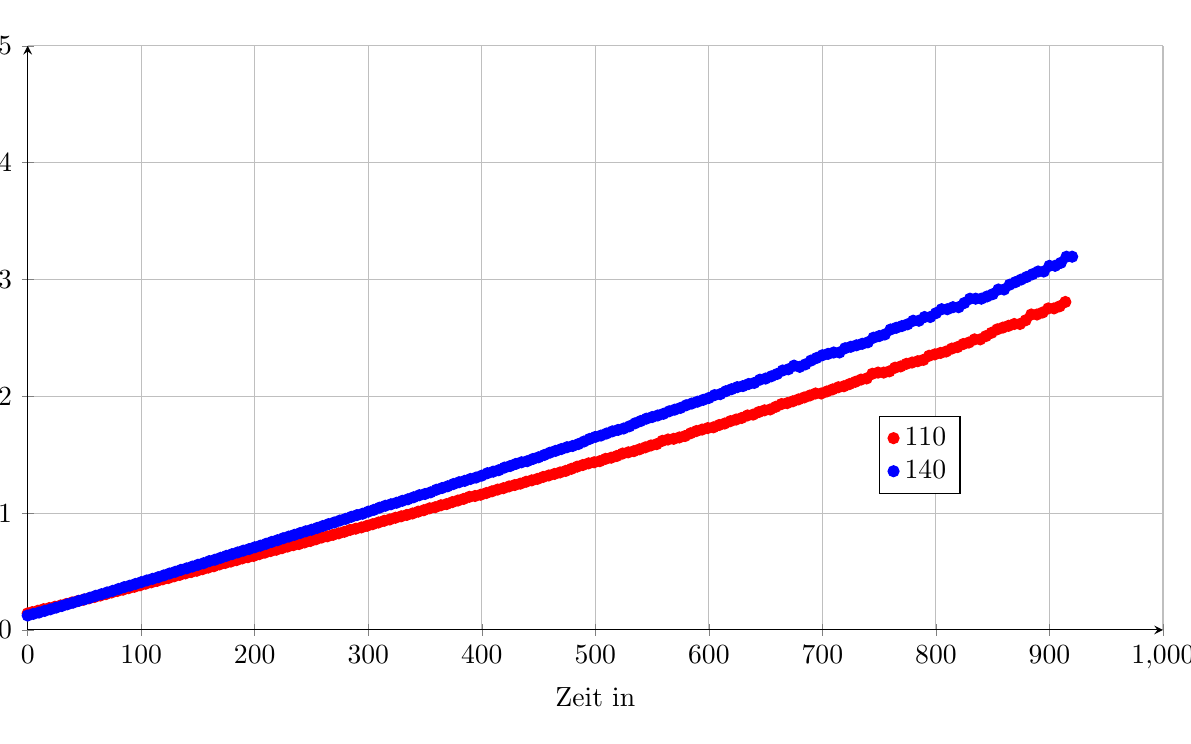
\begin{tikzpicture}[trim axis left, trim axis right]
				\begin{axis}[
					grid,
					axis lines = left,
					width = 16cm,
					height = 9cm,
					xmin = 0,
					xmax = 1000,
					ymin = 0,
					ymax = 5,
					xticklabel style={
						/pgf/number format/fixed,
						/pgf/number format/precision=5
					},
					%	ytick = {0,5,...,60},
					%	xtick = {0,1,2,...,15},
					ylabel={$\ln\left(\frac{c^\ast}{c^\ast-c}\right)$},
					%y label style={at={(0,0.5)}},
					xlabel={Zeit in \si{\second}},
					legend style={at={(0.75,0.3)},anchor=west},
					%	y dir = reverse,
					]			
					
					%diff regression
					%\addplot [color=black, mark=none, dashed, domain=50000:80000] {0.001081969*x-81.52975494};
					
					%int regression
					%\addplot [color=black, mark=none, dotted, domain=50000:80000] {0.000563159*x-44.87499061};
					
					
					%110
					\addplot [color=red, mark=*, only marks] coordinates{(0,0.14170003794847) (4,0.152254225627161) (9,0.164262375255557) (14,0.17777609442228) (19,0.187345545438431) (24,0.198395381625016) (29,0.209568682223141) (34,0.222289701824452) (39,0.235174633128312) (44,0.246768965909232) (49,0.258499305694721) (54,0.270368881250105) (59,0.282381037698109) (64,0.294539242177918) (69,0.306847089852515) (74,0.320876938062953) (79,0.333515336934676) (84,0.344706500895937) (89,0.357651665487974) (94,0.369117802575618) (99,0.382384995519667) (104,0.395830576229019) (109,0.40774561080689) (114,0.419804327127017) (119,0.433766159508786) (124,0.444366965495426) (129,0.458678479888682) (134,0.471371306687101) (139,0.484227314788635) (144,0.49537984673911) (149,0.506658161776817) (154,0.519979005752478) (159,0.533479692971381) (164,0.545198577084594) (169,0.561040492550252) (174,0.573088831066426) (179,0.585284104160245) (184,0.597629939982544) (189,0.612228739403697) (194,0.622788499618699) (199,0.633460959509471) (204,0.648596383574572) (209,0.661754468152083) (214,0.675087999021548) (219,0.686336711557419) (224,0.700004350286082) (229,0.713861384947509) (234,0.7255574247107) (239,0.735013759952735) (244,0.749368073404418) (249,0.761489433936763) (254,0.776231715673967) (259,0.791194588350679) (264,0.801295684337183) (269,0.81406725001667) (274,0.82700404104739) (279,0.84011038855269) (284,0.856068173991301) (289,0.86684994959459) (294,0.877749240052625) (299,0.891542562184961) (304,0.905528804159701) (309,0.919713439151657) (314,0.934102176603757) (319,0.9457641163516) (324,0.960535433671912) (329,0.972511624718628) (334,0.984632985250973) (339,0.996903077842787) (344,1.01245549085027) (349,1.02507395480948) (354,1.04107429615592) (359,1.05079884604792) (364,1.06721957626025) (369,1.07720302024443) (374,1.09406682629644) (379,1.1077656706546) (384,1.12165478281526) (389,1.13929192430137) (394,1.14643481181375) (399,1.15724572791797) (404,1.17184452733912) (409,1.18665961312426) (414,1.2016974904888) (419,1.21312618631242) (424,1.2285705087399) (429,1.24031232661658) (434,1.25219365450333) (439,1.26825825700714) (444,1.28047836834191) (449,1.29284966014446) (454,1.30958645249999) (459,1.32232547827742) (464,1.33522888311332) (469,1.34830096468068) (474,1.3615461914307) (479,1.37948389211736) (484,1.39774924009466) (489,1.41167057861327) (494,1.42578846015905) (499,1.43531234167031) (504,1.44492780036975) (509,1.46444061459333) (514,1.47434168557604) (519,1.48937956294058) (524,1.50978843457179) (529,1.52015122160734) (534,1.53062252147463) (539,1.54653797678053) (544,1.56271083602613) (549,1.57914956236929) (554,1.59026078779436) (559,1.61859129442059) (564,1.63015211682166) (569,1.63598303713246) (574,1.64774787871204) (579,1.65965278121836) (584,1.68389639282835) (589,1.70247277840129) (594,1.71505156060815) (599,1.72779058638558) (604,1.73422147671587) (609,1.75376607278884) (614,1.76701129953886) (619,1.78721400685638) (624,1.80091285121454) (629,1.81480196337521) (634,1.83600417102581) (639,1.84317266050442) (644,1.86499170789906) (649,1.87980679368421) (654,1.88729746541336) (659,1.91011214317953) (664,1.93345950717653) (669,1.94136468668364) (674,1.95736502803008) (679,1.97362554890186) (684,1.99015485085307) (689,2.00696196916945) (694,2.02405640252875) (699,2.02405640252875) (704,2.04144814524062) (709,2.05914772234002) (714,2.0771662278427) (719,2.08629871140597) (724,2.10481775917321) (729,2.12368624347759) (734,2.14291760540548) (739,2.15267378035085) (744,2.19267911496455) (749,2.20293561513173) (754,2.20293561513173) (759,2.21329840216728) (764,2.24504710048186) (769,2.25585801658608) (774,2.27783692330485) (779,2.28901022390298) (784,2.30030977915691) (789,2.31173847498053) (794,2.3468297947918) (799,2.35880598583852) (804,2.37092734637086) (809,2.38319743896268) (814,2.4081987411681) (819,2.42093776694553) (824,2.44691325334879) (829,2.46015848009881) (834,2.48718715248673) (839,2.48718715248673) (844,2.5149667165938) (849,2.54354008903786) (854,2.57295397424415) (859,2.58799185160869) (864,2.60325932373948) (869,2.61876351027545) (874,2.61876351027545) (879,2.65051220859003) (884,2.7001091497294) (889,2.7001091497294) (894,2.7172035830887) (899,2.75229490289997) (904,2.75229490289997) (909,2.77031340840265) (914,2.807354680083) };
					
					%140
					\addplot [color=blue, mark=*, only marks] coordinates{(0,0.123613955967177) (5,0.137494304999582) (10,0.148996029238594) (15,0.163235752049729) (20,0.176359299979537) (25,0.190996953213225) (30,0.204492434688109) (35,0.219550898562311) (40,0.233440010722978) (45,0.248944197258943) (50,0.261810707852193) (55,0.27630371515476) (60,0.292492442504678) (65,0.305935512761131) (70,0.321087317781734) (75,0.334923049634384) (80,0.350523990076863) (85,0.366372182316887) (90,0.379234095959295) (95,0.393904285707088) (100,0.408792898200839) (105,0.423906536010887) (110,0.437535367066493) (115,0.451352512619635) (120,0.467128475213803) (125,0.483157313489701) (130,0.497624111907455) (135,0.514153413858665) (140,0.527201129251141) (145,0.542324290825362) (150,0.557679678908556) (155,0.571311827698614) (160,0.589116452332121) (165,0.601164790848295) (170,0.617458430334396) (175,0.63402195600607) (180,0.64874356783143) (185,0.663685147829629) (190,0.678853369302801) (195,0.692040373584754) (200,0.707648271250745) (205,0.721223140341814) (210,0.737296965172875) (215,0.753633384492569) (220,0.767851633494848) (225,0.784699204067459) (230,0.799369393815253) (235,0.814258006309004) (240,0.829371644119052) (245,0.844717213793712) (250,0.85768756423634) (255,0.873477365968975) (260,0.889520490809551) (265,0.905825199834494) (270,0.91961852196683) (275,0.936425640283211) (280,0.950650631214558) (285,0.967992106251045) (290,0.982676657933967) (295,0.994581560440285) (300,1.01270894503284) (305,1.02807023019433) (310,1.0468207795397) (315,1.0627193656075) (320,1.07562277044341) (325,1.08869485201076) (330,1.1052789800263) (335,1.11874719707717) (340,1.13584163043647) (345,1.15323337314833) (350,1.16381548247887) (355,1.17810143972635) (360,1.19992048712099) (365,1.21473557290613) (370,1.22977345027067) (375,1.24889449171745) (380,1.26445900825856) (385,1.27629346590556) (390,1.292293807252) (395,1.30446434287226) (400,1.32092561992633) (405,1.34189074839138) (410,1.35468409985129) (415,1.36764324449379) (420,1.38962215121257) (425,1.40304517154471) (430,1.4212274906279) (435,1.43508452528932) (440,1.44443038770756) (445,1.46338830145217) (450,1.4778463846274) (455,1.49745485601578) (460,1.51745552272245) (465,1.53272299485324) (470,1.5482271813892) (475,1.56397553835734) (480,1.5746139365624) (485,1.590786795808) (490,1.61276570252678) (495,1.63523855837883) (500,1.65243095891921) (505,1.66405899691433) (510,1.68175857401373) (515,1.69977707951641) (520,1.71197235261022) (525,1.72431818843252) (530,1.74312752039002) (535,1.76876995100336) (540,1.78844271660206) (545,1.80851027965287) (550,1.82211593170865) (555,1.83590925384099) (560,1.84989549581573) (565,1.87124862028629) (570,1.88574162758886) (575,1.90044777497856) (580,1.92292063083062) (585,1.9381881029614) (590,1.95369228949737) (595,1.96944064646551) (600,1.98544098781195) (605,2.00993200782024) (610,2.01823081063494) (615,2.04354861861923) (620,2.06079042505374) (625,2.07833473470465) (630,2.08722368212189) (635,2.10524218762457) (640,2.11437467118784) (645,2.14228345930492) (650,2.15176220325946) (655,2.17099356518735) (660,2.19060203657573) (665,2.22075507474641) (670,2.2310115749136) (675,2.26242777114698) (680,2.25184566181645) (685,2.27312306026373) (690,2.30591288308672) (695,2.32838573893878) (700,2.35137525716348) (705,2.36307129692667) (710,2.37490575457367) (715,2.37490575457367) (720,2.41127339874455) (725,2.42369591874311) (730,2.43627470094996) (735,2.44901372672739) (740,2.4619171315633) (745,2.50165746021282) (750,2.5152631122686) (755,2.52905643440093) (760,2.57161604881973) (765,2.58621484824088) (770,2.60102993402602) (775,2.61606781139056) (780,2.64683947005732) (785,2.64683947005732) (790,2.6785881683719) (795,2.6785881683719) (800,2.71137799119489) (805,2.74527954287057) (810,2.74527954287057) (815,2.76267128558244) (820,2.76267128558244) (825,2.79838936818452) (830,2.83543063986486) (835,2.83543063986486) (840,2.83543063986486) (845,2.85447883483556) (850,2.87389692069266) (855,2.91390225530636) (860,2.91390225530636) (865,2.95557495170693) (870,2.97708115692789) (875,2.99906006364667) (880,3.02153291949873) (885,3.04452243772342) (890,3.06805293513362) (895,3.06805293513362) (900,3.11684309930305) (905,3.11684309930305) (910,3.14216090728734) (915,3.19480464077276) (920,3.19480464077276) };
					
					
					\legend{\SI{110}{\per \minute},\SI{140}{\per \minute}}
				\end{axis}
			\end{tikzpicture}
		}
		\caption{Integraler Ansatz zur Bestimmung des $\left[k_l*a\right]_{int}$}
		\label{dia:int}
	\end{center}
\end{figure}
\FloatBarrier

\textit{Regressionsgleichungen:}
\begin{flalign}
	y_{110} &=\SI{2,84E-03}{}*x+0,064\\
	y_{140} &= \SI{3,30E-03}{}*x+0,045
\end{flalign}

\begin{flalign}
	\label{gl:int}
	y &= m*x +n = y_{110} = \SI{2,84E-03}{}*x+0,064\\
	\left[k_l*a\right]_{int}&= m\\
	&= \underline{\SI{2,84E-03}{\per \second}}
\end{flalign}

\begin{figure}[h!]
	\begin{center}
		\resizebox{0.7\textwidth}{!}{
			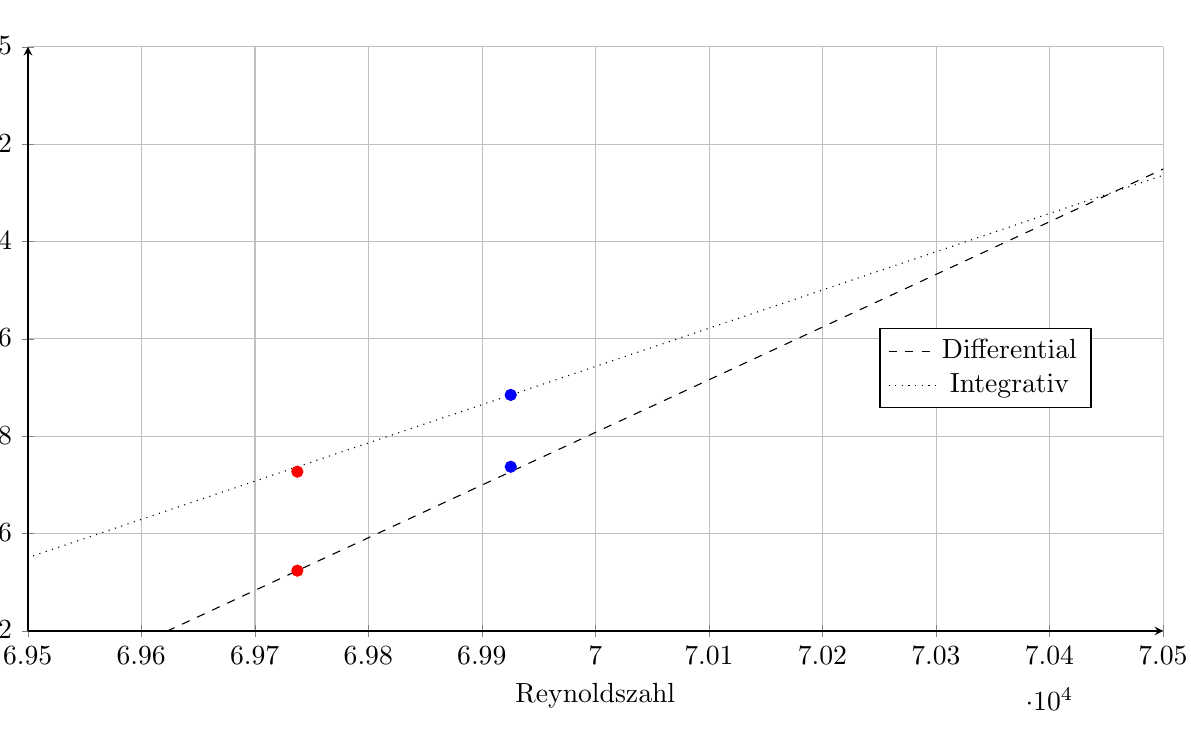
\begin{tikzpicture}[trim axis left, trim axis right]
				\begin{axis}[
					grid,
					axis lines = left,
					width = 16cm,
					height = 9cm,
					xmin = 69500,
					xmax = 70500,
					ymin = -6.2,
					ymax = -5,
					xticklabel style={
						/pgf/number format/fixed,
						/pgf/number format/precision=5
					},
					%	ytick = {0,5,...,60},
					%	xtick = {0,1,2,...,15},
					ylabel={$\ln\left(k_l*a\right)$},
					%y label style={at={(0,0.5)}},
					xlabel={Reynoldszahl},
					legend style={at={(0.75,0.45)},anchor=west},
					%	y dir = reverse,
					]			
					
						%diff regression
					\addplot [color=black, mark=none, dashed, domain=50000:80000] {0.001081969*x-81.52975494};
					
					%int regression
					\addplot [color=black, mark=none, dotted, domain=50000:80000] {0.00078545*x-60.63800152};
					
					
					%ln kla diff
					%\addplot [color=black, mark=*, only marks] coordinates{(50605.0296441165,-5.28698185688429) }; 
					\addplot [color=red, mark=*, only marks] coordinates{(69737.278852921,-6.076151355)};
					\addplot [color=blue, mark=*, only marks] coordinates{(69925.2308716865,-5.862679108)  };
					
				
					
					%ln kla int
					%\addplot [color=black, mark=*, only marks] coordinates{	(50605.0296441165,-5.57080627603783)}; 
					\addplot [color=red, mark=*, only marks] coordinates{ (69737.278852921,-5.872793017)};
					\addplot [color=blue, mark=*, only marks] coordinates{(69925.2308716865,-5.715051719) };
				 
					
					\legend{Differential,Integrativ}
				\end{axis}
			\end{tikzpicture}
		}
		\caption{Natürlich logarithmierter Stoffübertragungskoeffizient $k_l*a$ in Abhängigkeit der Reynoldszahl $Re$ für verschiedene Drehzahlen}
		\label{dia:reynolds}
	\end{center}
\end{figure}
\FloatBarrier

\textit{Regressionsgeraden:}
\begin{flalign*}
	y_{\text{diff}} &= \SI{1,08E-03}{}*x-81,53\\
	y_{\text{int}}&= \SI{7,85E-04}{}*x-60,64
\end{flalign*}

\subsection{Weitere Berechnungen}
In diesem Abschnitt werden Beispielrechnungen für weitere geforderte Werte wie der \textsc{Henry}-Konstante oder der effektiven Reaktionsgeschwindigkeit dargelegt. Es wird sich hierbei lediglich auf Vorberechnungen der differentiellen Methodik berufen.\\

\textbf{\textsc{Henry}-Konstante}\\
\begin{flalign}
	H \left[\si{\bar}\right] &= \frac{p_u*x_{\ce{O2}} }{c^\ast*n_{\ce{H2O}}*V_{\ce{H2O}}}\\
					H_{80}			&= \frac{\SI{1,013}{\bar}*0,21}{\SI{2,63E-04}{\mol \per \liter}*\SI{55,45}{\mol}*\SI{1}{\liter}}\\
										&= \underline{\SI{44937}{\bar}}
\end{flalign}

\textbf{$r_{\text{effektiv}}$, wenn Konzentration um 10\% bei Bulk absinkt}
\begin{flalign}
	r_{\text{effektiv}}&= k_l*a*\left(c^\ast-c^\ast*0,9\right)\\
	r_{\text{effektiv}, 110} &= \SI{2,30E-03}{\per \second}*\left(\SI{2,89E-04}{\mol \per \liter}-0,9*\SI{2,89E-04}{\mol \per \liter}\right)\\
									&= \underline{\SI{6,63E-08}{\mol \per \liter \per \second}}
\end{flalign}

\textbf{RZA für 100 \% Stoffumsatz bei $M = \SI{100}{\gram \per \mole}$}
\begin{flalign}
	RZA &= r_{\text{effektiv}} * \left(M+M_{\ce{O2}}\right)\\
	RZA_{110} &= \SI{6,63E-08}{\mol \per \liter \per \second}*\left(\SI{100}{\gram \per \mol}+\SI{32}{\gram \per \mol}\right)\\
					&= \underline{\SI{8,76E-06}{\gram \per \liter \per \second}}
\end{flalign}

% Table generated by Excel2LaTeX from sheet 'Daten'
\begin{table}[h!]
	\renewcommand*{\arraystretch}{1.2}
	\centering
	\rowcolors{2}{white}{gray!25}
	\caption{Zusammenfassende Werte}
	\label{tab: uebersicht}
	\resizebox{12cm}{!}{
		\begin{tabulary}{1.2\textwidth}{C|C|C|C}
			\hline
			   \textbf{Betrachteter Wert}     & \SI{80}{\per\minute} & \SI{110}{\per\minute} & \SI{140}{\per\minute} \\
			   $\left[k_l*a\right]_{diff} \, \left[\si{\per \second}\right]$      &       \SI{5,06E-03}{}               &          \SI{2,30E-03}{}              &         \SI{2,82E-03}{}                \\
			         $c^\ast_{diff} \,  \left[\si{\milli \mol\per \liter}\right]$     &         \SI{2,63E-01}{}               &           \SI{2,89E-01}{}              &          \SI{2,89E-01}{}               \\
			    $\left[k_l*a\right]_{int} \, \left[\si{\per \second}\right]$     	&         \SI{3,81E-03}{}               &      \SI{2,84E-03}{}                   &         \SI{3,30E-03}{}                \\
			         $c^\ast_{int} \, \left[\si{\milli \mol\per \liter}\right]$           		&        \SI{2,72E-01}{}                &         \SI{2,74E-01}{}                &      \SI{2,82E-01}{}                   \\
			 				\textsc{Reynoldszahl}									&        \SI{5,06E+04}{}                &               \SI{6,97E+04}{}               &       \SI{6,99E+04}{}             \\
			\textsc{Henry}-Konstante $ \left[\si{\bar}\right]$ &       \SI{44937}{}                   &                     \SI{40837}{}        &         \SI{40751}{}            \\
			      $r_{\text{effektiv}} \, \left[\si{\mol \per \liter\per \second}\right]$       			&       \SI{1,33E-07}{}                &             \SI{6,63E-08}{}            &     \SI{8,15E-08}{}                    \\
			              $RZA \, \left[\si{\gram \per \liter\per \second}\right]$               				&       \SI{1,75E-05}{}                 &            \SI{8,76E-06}{}             &       \SI{1,08E-05}{}                  \\
			         \textbf{ Plausibel ?}        				&      eher nicht      &          ja           &          ja           \\ \hline
		\end{tabulary}
 	}
\end{table}%
\FloatBarrier